\subsection{CPUとの比較・ハードウエア実装の成果}
今回の実験では、当初\ref{sec:goal}で設定した目標のうち、1. と2. を実行することができた。
表~\ref{tab:time}と表~\ref{tab:compile}に示した結果より、
\begin{itemize}
    \item 並列度1・10MHzで動作させた場合、19.5ms程度
    \item 並列度3・10MHzで動作させた場合、6.5ms程度
\end{itemize}
で局所最適解に到達することができるプログラムを実装することができた。
今回の手法に相当するプログラムをPythonで実装し実行した際、局所最適解に到達する所要時間は平均して45msであったので、約7倍の高速化を達成することができた。

\subsection{並列度に対する考察}
並列度を上げることで、局所最適解に到達するまでの時間は線形に減少した。最終的に並列度は3で実行させることになったが、これ以上並列度を上げることはリソースの関係でできなかった。
これは\ref{sec:compile}で示した通り使用ロジック数が並列度にたいし指数関数的に増加するためであるが、

頂点情報・ロック配列にランダムアクセスする要素が多数存在する点が要因であると考えられる。
各交換モジュールには最大6点の情報を渡すが、これらの情報はすべて山登りモジュールで計算する。
頂点配列・ロック配列に並列度×定数個同時にランダムアクセスを行い、相互に制約をかけあって干渉しているため使用ロジック数が増加したものと考えられる。

対策として、山登りモジュールでの近傍生成を交換モジュールごとに行うのではなく、交換モジュールとは非同期に行ってFIFOに格納し、
各交換モジュールがFIFOからフェッチする構造にするという手法が考えられる。一つ一つのデータに対する同時ランダムアクセス数が現象するため、使用ロジック数の爆発的な増加を抑えることができると考える。
また、この方法によって、近傍生成・交換判定のそれぞれが互いの進行に律速されることなく独立に処理を進めることができるので、処理待ちのモジュールがなくなり、並列度を上げることができると考えられる。

\subsection{最大動作周波数に関する分析・追加検証}\label{sec:frequency}
\ref{sec:distance}節で述べたように、実験時間中に実装した距離計算モジュールではニュートン法を5クロックに分割しパイプライン化した。
当初1クロックで計算していた際は最大周波数が4MHz程度しか出なかったのに対し、分割によって12MHz程度に改善した。
これはステージ分割によって、1クロックあたりの除算の回数が3回から最大1回に減少したことによるものと考えられる。

また、ユークリッド距離のかわりに計算コストが極めて軽いマンハッタン距離を用いたところ、47.8MHzで動作可能であったため、
距離計算モジュール、特に除算が最大動作周波数を大幅に下げていることが判明した。

除算は、加算減算乗算に比べ非常に遅く、一般的なプロセッサでは、数十クロックかけることもある。\cite{InfographicsOperationCosts2016}したがって、除算を含むモジュールは、動作周波数を大きく下げる要因となる。
この問題を是正するために、以下の2つの方法を考え、それぞれ実験期間終了後に検証した。
\begin{itemize}
    \item 方法1: 除算の高速化
    \item 方法2: 除算を含まない距離計算方法の実装
\end{itemize}
\subsubsection{方法1: 除算の高速化}
今回除算を必要とするのは、二乗距離の平方根を計算する部分であり、各座標が$[0,255]$の8bit整数であることから、二乗距離は18bitで表現可能である。
現状32bitに対する除算を用いていたことから、除算の精度を下げることで高速化を図ることができると考えた。

除算の精度を18bitに下げたところ、最大動作周波数は21.4MHzまで改善した。

\subsubsection{方法2: 除算を含まない距離計算方法の実装}
今回の平方根計算ではニュートン法を用いたが、平方根計算には除算が不要な方法も存在する。
その中でも、二分法を用いて距離計算する方法を検討する。
ある値$t$と$\sqrt{x}$の大小関係は、$t^2$と$x$の大小関係と同じであることを利用し、上位ビットから順に1ビットずつ決定することができる。

例えば、$x=100 (\sqrt{100}=10)$に対して、
\begin{itemize}
    \item $t=10000_{(2)}=16$のとき、$t^2=100000000_{(2)}=256$より、$t^2>x$であるため、$t$の5ビット目は0となる。
    \item $t=01000_{(2)}=8$のとき、$t^2=010000000_{(2)}=64$より、$t^2<x$であるため、$t$の4ビット目は1となる。
    \item $t=01100_{(2)}=12$のとき、$t^2=011000000_{(2)}=144$より、$t^2>x$であるため、$t$の3ビット目は0となる。
    \item $t=01010_{(2)}=10$のとき、$t^2=010100100_{(2)}=100$より、$t^2=x$であるため、$t$の2ビット目は1となる。
    \item $t=01011_{(2)}=11$のとき、$t^2=010110100_{(2)}=121$より、$t^2>x$であるため、$t$の1ビット目は0となる。
\end{itemize}
以上より、$\sqrt{100}=01010_{(2)}=10$が求まる。二分法では、$O(\log x)$回の乗算と比較で平方根を求めることができる。

今回、ユークリッド距離は9bitで表現可能なので、9回の乗算と比較で整数範囲で正確な距離を求めることができる。

この方法を用いて図~\ref{fig:distance_binary}のように11クロックでパイプライン化して計算するよう変更を加えると、最大動作周波数は48.5MHzまで改善した。
これはマンハッタン距離を用いた場合と同等の値であるから、周波数的なボトルネックを除去することができたと考えられる。
処理を分割したことから距離1つあたりの所要クロックは増加したが、パイプライン化によって並列度も上がっている。
したがって総クロック数が大幅に増えるというわけではなく、周波数増加による高速化効果が上回っていると思われる。

\begin{figure}[h]
    \begin{center}
        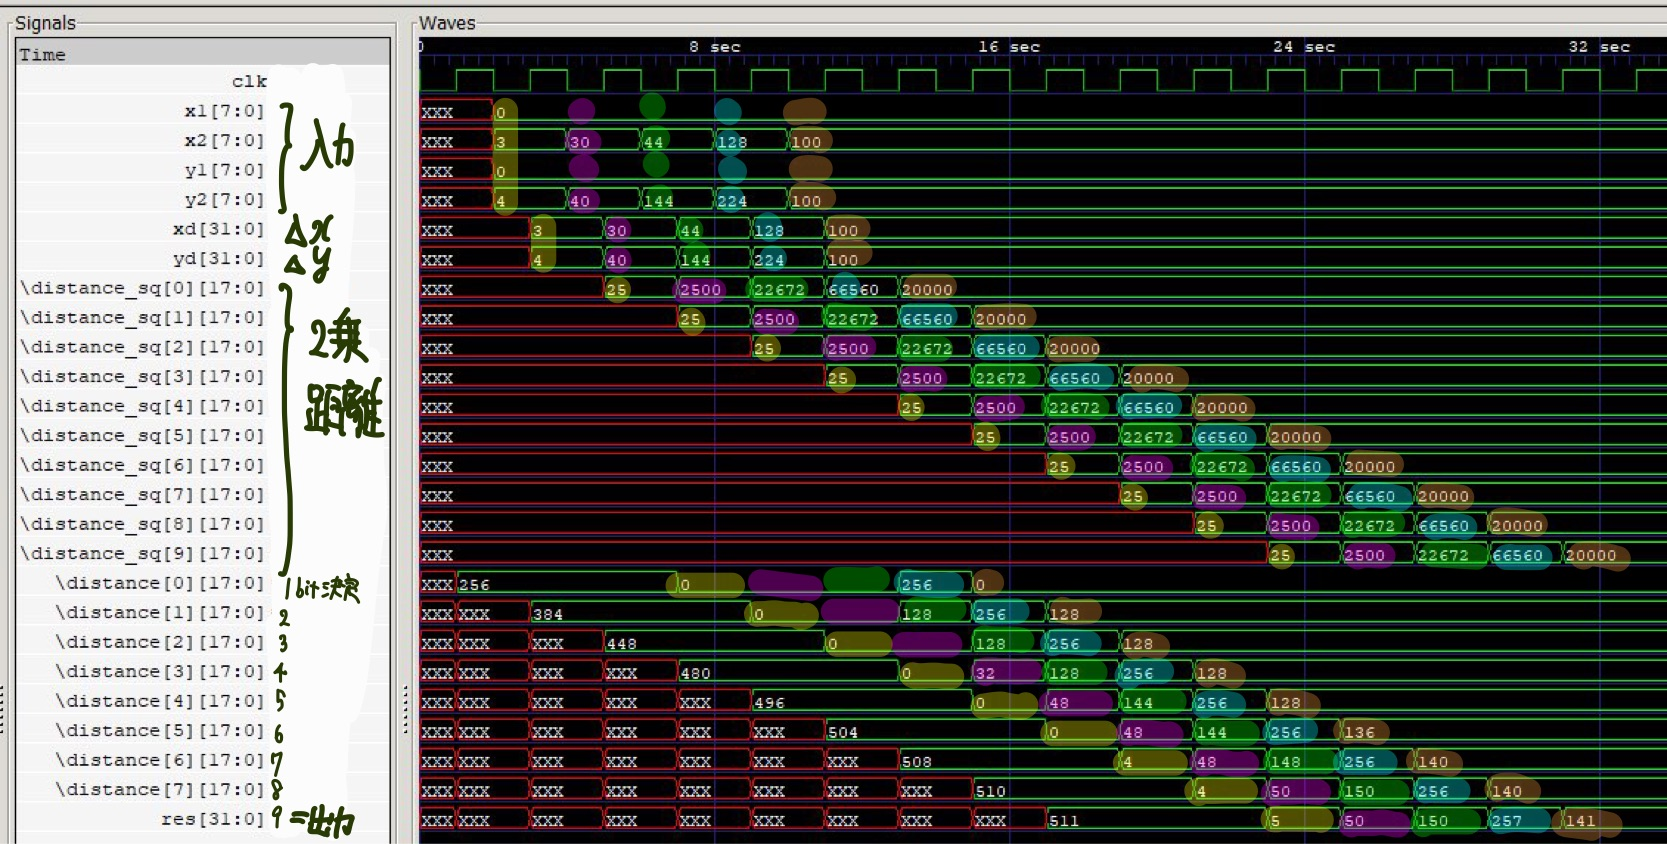
\includegraphics[width=15cm]{figure/distance_binary.jpg}
        \caption{距離計算モジュールの二分法による実装とパイプライン化}\label{fig:distance_binary}
    \end{center}
\end{figure}

\subsection{総括・今後の展望}
今回の実験では、巡回セールスマン問題に対し、CPUより高速に局所最適解に陥るハードウエアプログラムを作成することができ、並列性というハードウエア実装の優位性を確認することはできた。
しかしながら局所最適解以降の処理については実装しておらず、十分な精度の解を得ることはできなかった。
最大の要因としては実装時間不足が挙げられるが、山登り法を実装してから3回分の実験を実機上でのバグ修正に費やしてしまったのが大きなロスとなった。
結局、バグの原因は「低周波数でしか機能しない回路に50MHzのクロックを渡していたこと」であり、PLLを挟むだけで解決した。

ハードウエアでのアルゴリズム実装においては、CPUではあまり意識しない部分での最適化が重要であり、大きな差を生むということがわかった。
成果としては満足だが、まだ発展途上であると思うので、今後時間があれば、
\begin{itemize}
    \item 温度パラメータと確率的な近傍遷移を実装して局所最適解に陥らないようにする(焼き鈍し法)
    \item 2-opt法など、本質的に異質な遷移を実装し、局所最適解でランダムに実行することでより良い解を得る(反復局所探索法)
    \item 近傍選択モジュールと交換モジュールの非同期化による並列度の向上
    \item 三角不等式など数理的手法を活用した交換判定モジュールの枝刈り高速化
    \item VGA出力によるリアルタイム可視化
\end{itemize}
などを実装・検証していきたいと考えている。